% Options for packages loaded elsewhere
\PassOptionsToPackage{unicode}{hyperref}
\PassOptionsToPackage{hyphens}{url}
\PassOptionsToPackage{dvipsnames,svgnames,x11names}{xcolor}
\PassOptionsToPackage{space}{xeCJK}
%
\documentclass[
  letterpaper,
]{LegrandOrangeBook}

%%%%%%%%%%%%%%%%%%%%%%%%%%%%%%%%%%%%%%%%%%%%%%%%%%%%%%%%%%%%%%%%%%%%%%%
%
% Settings for Legrand Orange Book document class and other decorations
%
%%%%%%%%%%%%%%%%%%%%%%%%%%%%%%%%%%%%%%%%%%%%%%%%%%%%%%%%%%%%%%%%%%%%%%%

  \definecolor{ocre}{RGB}{26, 69, 135}

  \chapterimage{non-generated/banner.jpg} % Chapter heading image
\chapterspaceabove{6.5cm} % Default whitespace from the top of the page to the chapter title on chapter pages
\chapterspacebelow{6.75cm} % Default amount of vertical whitespace from the top margin to the start of the text on chapter pages

% title page

  \definecolor{titlepagecolor}{RGB}{0, 128, 128}

% The following code is borrowed from: https://tex.stackexchange.com/a/86310/10898

\newcommand\titlepagedecoration{%
\begin{tikzpicture}[remember picture,overlay,shorten >= -10pt]

\coordinate (aux1) at ([yshift=-15pt]current page.north east);
\coordinate (aux2) at ([yshift=-410pt]current page.north east);
\coordinate (aux3) at ([xshift=-4.5cm]current page.north east);
\coordinate (aux4) at ([yshift=-150pt]current page.north east);

\begin{scope}[titlepagecolor!40,line width=12pt,rounded corners=12pt]
\draw
  (aux1) -- coordinate (a)
  ++(225:5) --
  ++(-45:5.1) coordinate (b);
\draw[shorten <= -10pt]
  (aux3) --
  (a) --
  (aux1);
\draw[opacity=0.6,titlepagecolor,shorten <= -10pt]
  (b) --
  ++(225:2.2) --
  ++(-45:2.2);
\end{scope}
\draw[titlepagecolor,line width=8pt,rounded corners=8pt,shorten <= -10pt]
  (aux4) --
  ++(225:0.8) --
  ++(-45:0.8);
\begin{scope}[titlepagecolor!70,line width=6pt,rounded corners=8pt]
\draw[shorten <= -10pt]
  (aux2) --
  ++(225:3) coordinate[pos=0.45] (c) --
  ++(-45:3.1);
\draw
  (aux2) --
  (c) --
  ++(135:2.5) --
  ++(45:2.5) --
  ++(-45:2.5) coordinate[pos=0.3] (d);   
\draw 
  (d) -- +(45:1);
\end{scope}
\end{tikzpicture}%
}

% add the title page decoration
\makeatletter
\def\@endpart{\titlepagedecoration\vfil\newpage
\if@tempswa\twocolumn\fi}
\makeatother

\usepackage{amsmath,amssymb}
\usepackage{lmodern}
\usepackage{setspace}
\usepackage{iftex}
\ifPDFTeX
  \usepackage[T1]{fontenc}
  \usepackage[utf8]{inputenc}
  \usepackage{textcomp} % provide euro and other symbols
\else % if luatex or xetex
  \usepackage{unicode-math}
  \defaultfontfeatures{Scale=MatchLowercase}
  \defaultfontfeatures[\rmfamily]{Ligatures=TeX,Scale=1}
  \ifXeTeX
    \usepackage{xeCJK}
    \setCJKmainfont[]{Noto Serif CJK SC}
  \fi
  \ifLuaTeX
    \usepackage[]{luatexja-fontspec}
    \setmainjfont[]{Noto Serif CJK SC}
  \fi
\fi
% Use upquote if available, for straight quotes in verbatim environments
\IfFileExists{upquote.sty}{\usepackage{upquote}}{}
\IfFileExists{microtype.sty}{% use microtype if available
  \usepackage[]{microtype}
  \UseMicrotypeSet[protrusion]{basicmath} % disable protrusion for tt fonts
}{}
\makeatletter
\@ifundefined{KOMAClassName}{% if non-KOMA class
  \IfFileExists{parskip.sty}{%
    \usepackage{parskip}
  }{% else
    \setlength{\parindent}{0pt}
    \setlength{\parskip}{6pt plus 2pt minus 1pt}}
}{% if KOMA class
  \KOMAoptions{parskip=half}}
\makeatother
\usepackage{xcolor}
\IfFileExists{xurl.sty}{\usepackage{xurl}}{} % add URL line breaks if available
\IfFileExists{bookmark.sty}{\usepackage{bookmark}}{\usepackage{hyperref}}
\hypersetup{
  pdftitle={Readability Studio 2024.0.1},
  pdfauthor={Blake Madden},
  colorlinks=true,
  linkcolor={black},
  filecolor={Maroon},
  citecolor={black},
  urlcolor={Blue},
  pdfcreator={LaTeX via pandoc}}
\urlstyle{same} % disable monospaced font for URLs
\usepackage{color}
\usepackage{fancyvrb}
\newcommand{\VerbBar}{|}
\newcommand{\VERB}{\Verb[commandchars=\\\{\}]}
\DefineVerbatimEnvironment{Highlighting}{Verbatim}{commandchars=\\\{\}}
% Add ',fontsize=\small' for more characters per line
\usepackage{framed}
\definecolor{shadecolor}{RGB}{241,243,245}
\newenvironment{Shaded}{\begin{snugshade}}{\end{snugshade}}
\newcommand{\AlertTok}[1]{\textcolor[rgb]{0.68,0.00,0.00}{#1}}
\newcommand{\AnnotationTok}[1]{\textcolor[rgb]{0.37,0.37,0.37}{#1}}
\newcommand{\AttributeTok}[1]{\textcolor[rgb]{0.40,0.45,0.13}{#1}}
\newcommand{\BaseNTok}[1]{\textcolor[rgb]{0.68,0.00,0.00}{#1}}
\newcommand{\BuiltInTok}[1]{\textcolor[rgb]{0.00,0.23,0.31}{#1}}
\newcommand{\CharTok}[1]{\textcolor[rgb]{0.13,0.47,0.30}{#1}}
\newcommand{\CommentTok}[1]{\textcolor[rgb]{0.37,0.37,0.37}{#1}}
\newcommand{\CommentVarTok}[1]{\textcolor[rgb]{0.37,0.37,0.37}{\textit{#1}}}
\newcommand{\ConstantTok}[1]{\textcolor[rgb]{0.56,0.35,0.01}{#1}}
\newcommand{\ControlFlowTok}[1]{\textcolor[rgb]{0.00,0.23,0.31}{\textbf{#1}}}
\newcommand{\DataTypeTok}[1]{\textcolor[rgb]{0.68,0.00,0.00}{#1}}
\newcommand{\DecValTok}[1]{\textcolor[rgb]{0.68,0.00,0.00}{#1}}
\newcommand{\DocumentationTok}[1]{\textcolor[rgb]{0.37,0.37,0.37}{\textit{#1}}}
\newcommand{\ErrorTok}[1]{\textcolor[rgb]{0.68,0.00,0.00}{#1}}
\newcommand{\ExtensionTok}[1]{\textcolor[rgb]{0.00,0.23,0.31}{#1}}
\newcommand{\FloatTok}[1]{\textcolor[rgb]{0.68,0.00,0.00}{#1}}
\newcommand{\FunctionTok}[1]{\textcolor[rgb]{0.28,0.35,0.67}{#1}}
\newcommand{\ImportTok}[1]{\textcolor[rgb]{0.00,0.46,0.62}{#1}}
\newcommand{\InformationTok}[1]{\textcolor[rgb]{0.37,0.37,0.37}{#1}}
\newcommand{\KeywordTok}[1]{\textcolor[rgb]{0.00,0.23,0.31}{\textbf{#1}}}
\newcommand{\NormalTok}[1]{\textcolor[rgb]{0.00,0.23,0.31}{#1}}
\newcommand{\OperatorTok}[1]{\textcolor[rgb]{0.37,0.37,0.37}{#1}}
\newcommand{\OtherTok}[1]{\textcolor[rgb]{0.00,0.23,0.31}{#1}}
\newcommand{\PreprocessorTok}[1]{\textcolor[rgb]{0.68,0.00,0.00}{#1}}
\newcommand{\RegionMarkerTok}[1]{\textcolor[rgb]{0.00,0.23,0.31}{#1}}
\newcommand{\SpecialCharTok}[1]{\textcolor[rgb]{0.37,0.37,0.37}{#1}}
\newcommand{\SpecialStringTok}[1]{\textcolor[rgb]{0.13,0.47,0.30}{#1}}
\newcommand{\StringTok}[1]{\textcolor[rgb]{0.13,0.47,0.30}{#1}}
\newcommand{\VariableTok}[1]{\textcolor[rgb]{0.07,0.07,0.07}{#1}}
\newcommand{\VerbatimStringTok}[1]{\textcolor[rgb]{0.13,0.47,0.30}{#1}}
\newcommand{\WarningTok}[1]{\textcolor[rgb]{0.37,0.37,0.37}{\textit{#1}}}
\usepackage{longtable,booktabs,array}
\usepackage{calc} % for calculating minipage widths
% Correct order of tables after \paragraph or \subparagraph
\usepackage{etoolbox}
\makeatletter
\patchcmd\longtable{\par}{\if@noskipsec\mbox{}\fi\par}{}{}
\makeatother
% Allow footnotes in longtable head/foot
\IfFileExists{footnotehyper.sty}{\usepackage{footnotehyper}}{\usepackage{footnote}}
\makesavenoteenv{longtable}
\usepackage{graphicx}
\makeatletter
\newsavebox\pandoc@box
\newcommand*\pandocbounded[1]{% scales image to fit in text height/width
  \sbox\pandoc@box{#1}%
  \Gscale@div\@tempa{\textheight}{\dimexpr\ht\pandoc@box+\dp\pandoc@box\relax}%
  \Gscale@div\@tempb{\linewidth}{\wd\pandoc@box}%
  \ifdim\@tempb\p@<\@tempa\p@\let\@tempa\@tempb\fi% select the smaller of both
  \ifdim\@tempa\p@<\p@\scalebox{\@tempa}{\usebox\pandoc@box}%
  \else\usebox{\pandoc@box}%
  \fi%
}
% Set default figure placement to htbp
\def\fps@figure{htbp}
\makeatother
\setlength{\emergencystretch}{3em} % prevent overfull lines
\providecommand{\tightlist}{%
  \setlength{\itemsep}{0pt}\setlength{\parskip}{0pt}}
\setcounter{secnumdepth}{5}
% Make \paragraph and \subparagraph free-standing
\ifx\paragraph\undefined\else
  \let\oldparagraph\paragraph
  \renewcommand{\paragraph}[1]{\oldparagraph{#1}\mbox{}}
\fi
\ifx\subparagraph\undefined\else
  \let\oldsubparagraph\subparagraph
  \renewcommand{\subparagraph}[1]{\oldsubparagraph{#1}\mbox{}}
\fi
% LaTeX packages that we will need

% TOC
% make the space for numbers wide enough so that the section names
% don't overlap the numbers.
\makeatletter
\renewcommand{\l@section}{\@dottedtocline{1}{1.5em}{3em}}
\renewcommand{\l@subsection}{\@dottedtocline{2}{4.0em}{3.6em}}
\renewcommand{\l@subsubsection}{\@dottedtocline{3}{7.4em}{4.5em}}
\renewcommand{\l@figure}{\@dottedtocline{1}{0em}{3em}}
\let\l@table\l@figure
\makeatother

% index
\usepackage{imakeidx}
\makeindex[intoc=true,columnseprule=true,
           options= -s latex/indexstyles.ist]
\newcommand{\idxit}[1]{{\it #1}}

% to create a "see also" that appears at the bottom of the
% subentries and with no page number, do the following:
% \index{Main entry!zzzzz@\igobble|seealso{Other item}}
\def\igobble#1{}

\usepackage{changepage}
\usepackage{mdframed}
\usepackage{bbding}
\usepackage{amsthm}
\usepackage{xeCJK}
\usepackage[all]{nowidow}
\usepackage{menukeys}
\usepackage{amsmath}
\usepackage{color}
\usepackage{xcolor}
\usepackage{listings}
\usepackage[most]{tcolorbox}
\usepackage{wrapfig}
\usepackage{url}
\usepackage{setspace}
\usepackage{lettrine}
\usepackage{caption}
\usepackage{stringstrings}

% table packages
\usepackage{booktabs}
\usepackage{longtable,tabu}
\usepackage{makecell}
\usepackage{threeparttable}
\usepackage{threeparttablex}
\usepackage{colortbl}
\usepackage{float}

% fonts and graphics
\usepackage{fontawesome5}
\usepackage{fontspec}
\usepackage{adforn}
\usepackage{overpic}
\usepackage{tikz}
\usepackage{ragged2e}

% words to not hyphenate
\hyphenation{Readability}
\hyphenation{Studio}
\hyphenation{LibreOffice}
\hyphenation{Microsoft}
\hyphenation{ExportAll}
\hyphenation{FORTRAN}
\hyphenation{COBOL}
\hyphenation{FORCAST}
\hyphenation{histograms}
\hyphenation{otherwise}

% MLA requirements
\usepackage[letterpaper, margin=1in]{geometry}

% make the page headers fancy
\usepackage{fancyhdr}

\pagestyle{fancy}
\fancyhf{}
\fancyhead[LO]{\nouppercase{\leftmark}}
\fancyhead[RE]{\nouppercase{\rightmark}}
\fancyhead[LE,RO]{\thepage}

% color box that displays a quote in fancy format
% https://tex.stackexchange.com/questions/16964/block-quote-with-big-quotation-marks
\usetikzlibrary{shadows,calc,scopes,backgrounds}
\usepackage{tikzpagenodes}
\makeatletter

\tikzset{%
  fancy quotes/.style={
    text width=\fq@width pt,
    align=justify,
    inner sep=1em,
    anchor=north west,
    minimum width=\linewidth,
  },
  fancy quotes width/.initial={.8\linewidth},
  fancy quotes marks/.style={
    scale=8,
    text=white,
    inner sep=0pt,
  },
  fancy quotes opening/.style={
    fancy quotes marks,
  },
  fancy quotes closing/.style={
    fancy quotes marks,
  },
  fancy quotes background/.style={
    show background rectangle,
    inner frame xsep=0pt,
    background rectangle/.style={
      fill=gray!25,
      rounded corners,
    },
  }
}

\newenvironment{fancyquotes}[1][]{%
\noindent
\tikzpicture[fancy quotes background]
\node[fancy quotes opening,anchor=north west] (fq@ul) at (0,0) {``};
\tikz@scan@one@point\pgfutil@firstofone(fq@ul.east)
\pgfmathsetmacro{\fq@width}{\linewidth - 2*\pgf@x}
\node[fancy quotes,#1] (fq@txt) at (fq@ul.north west) \bgroup}
{\egroup;
\node[overlay,fancy quotes closing,anchor=east] at (fq@txt.south east) {''};
\endtikzpicture}

\makeatother

\makeatletter
\def\thm@space@setup{%
  \thm@preskip=8pt plus 2pt minus 4pt
  \thm@postskip=\thm@preskip
}
\makeatother
\raggedbottom

%% Provides Creative Commons Icons
\usepackage{ccicons}

% Float features
%%%%%%%%%%%%%%%%%%%%%%%%%%%%%%%%%%%%%%%%

% don't float anything
\floatplacement{table}{H}
\floatplacement{figure}{H}

% helps reduce images from floating also
\renewcommand{\topfraction}{.85}
\renewcommand{\bottomfraction}{.7}
\renewcommand{\textfraction}{.15}
\renewcommand{\floatpagefraction}{.66}
\setcounter{topnumber}{3}
\setcounter{bottomnumber}{3}
\setcounter{totalnumber}{4}

% the warning, note, and tip color boxes
%%%%%%%%%%%%%%%%%%%%%%%%%%%%%%%%%%%%%%%%

% colors that can be used
\definecolor{lightgray}{RGB}{215,215,215}
\definecolor{ultralightgray}{RGB}{241,241,241}
\definecolor{lightyellow}{RGB}{252,248,227}
\definecolor{lightpink}{RGB}{255,207,219}
\definecolor{lightblue}{RGB}{232,244,248}
\definecolor{mediumblue}{RGB}{28,77,93}

% Tip box
\newenvironment{tipsection}
    {
    \begin{tcolorbox}[colframe=lightgray,colback=lightyellow,arc=3mm]
    \faLightbulb[regular] \textbf{Tip} \newline
    }
    {
    \end{tcolorbox}
    }

% Note box
\newenvironment{notesection}
    {
    \begin{tcolorbox}[colframe=mediumblue,colback=lightblue,coltext=mediumblue,arc=3mm]
    \faEdit[regular] \textbf{Note} \newline
    }
    {
    \end{tcolorbox}
    }

% Warning box
\newenvironment{warningsection}
    {
    \begin{tcolorbox}[colframe=lightgray,colback=lightpink,arc=3mm]
    \faExclamationTriangle[solid] \textbf{{Warning} } \newline
    }
    {
    \end{tcolorbox}
    }

% A light gray box for related program options (e.g., a radio button group, a combobox and its values, etc.).
\newenvironment{optionssection}
    {
    \begin{tcolorbox}[colframe=lightgray,colback=ultralightgray,sharp corners=all,parbox=false]
    }
    {
    \end{tcolorbox}
    }

% Title to add at the top of an optionssection.
\newenvironment{optionssectiontitle}
    {
    \begin{tcolorbox}[colframe=lightgray,colback=lightgray]
    \bfseries
    }
    {
    \end{tcolorbox}
    }

%% theming
\newenvironment{darkmode}
  {
  \begin{mdframed}[backgroundcolor=black]
  \color{white}
  }
  {
  \end{mdframed}
  }

% pseudo glossary features
\newenvironment{glsentry}
  {
  \begin{minipage}{\textwidth}
  }
  {
  \end{minipage}
  }

\newenvironment{glsterm}
  {
  \bfseries
  }
  {
  }

\newenvironment{glsdef}
  {
  \noindent
  \flushleft
  \begin{adjustwidth}{2cm}{}
  }
  {
  \end{adjustwidth}
  }
\usepackage{booktabs}
\usepackage{longtable}
\usepackage{array}
\usepackage{multirow}
\usepackage{wrapfig}
\usepackage{float}
\usepackage{colortbl}
\usepackage{pdflscape}
\usepackage{tabu}
\usepackage{threeparttable}
\usepackage{threeparttablex}
\usepackage[normalem]{ulem}
\usepackage{makecell}
\usepackage{xcolor}
\makeatletter
\@ifpackageloaded{bookmark}{}{\usepackage{bookmark}}
\makeatother
\makeatletter
\@ifpackageloaded{caption}{}{\usepackage{caption}}
\AtBeginDocument{%
\ifdefined\contentsname
  \renewcommand*\contentsname{Table of contents}
\else
  \newcommand\contentsname{Table of contents}
\fi
\ifdefined\listfigurename
  \renewcommand*\listfigurename{List of Figures}
\else
  \newcommand\listfigurename{List of Figures}
\fi
\ifdefined\listtablename
  \renewcommand*\listtablename{List of Tables}
\else
  \newcommand\listtablename{List of Tables}
\fi
\ifdefined\figurename
  \renewcommand*\figurename{Figure}
\else
  \newcommand\figurename{Figure}
\fi
\ifdefined\tablename
  \renewcommand*\tablename{Table}
\else
  \newcommand\tablename{Table}
\fi
}
\@ifpackageloaded{float}{}{\usepackage{float}}
\floatstyle{ruled}
\@ifundefined{c@chapter}{\newfloat{codelisting}{h}{lop}}{\newfloat{codelisting}{h}{lop}[chapter]}
\floatname{codelisting}{Listing}
\newcommand*\listoflistings{\listof{codelisting}{List of Listings}}
\makeatother
\makeatletter
\makeatother
\makeatletter
\@ifpackageloaded{caption}{}{\usepackage{caption}}
\@ifpackageloaded{subcaption}{}{\usepackage{subcaption}}
\makeatother
\ifLuaTeX
  \usepackage{selnolig}  % disable illegal ligatures
\fi
\usepackage[style=mla,maxbibnames=4]{biblatex}
\setlength\bibitemsep{\baselineskip}
\nocite{*}

\title{Readability Studio 2024.0.1}
\usepackage{etoolbox}
\makeatletter
\providecommand{\subtitle}[1]{% add subtitle to \maketitle
  \apptocmd{\@title}{\par {\large #1 \par}}{}{}
}
\makeatother
\subtitle{System Administrator Manual}
\author{Blake Madden}
\date{2025}

\def\theauthor{Blake Madden}
\def\thedate{2025}
\def\thetitle{Readability Studio 2024.0.1}
\def\thesubtitle{System Administrator Manual}
\def\authorbio{}
\def\thepublisher{Oleander Software, Ltd.}
\def\thepublishercities{\hspace{1cm}Dayton}
\def\trademark{\textit{Readability
Studio}\textsuperscript{\tiny\textregistered}}

% Either shows a logo for the publisher or their name in bold
\def\thepublisherlogo{\large \textbf{\thepublisher}}

% Optional watermark (e.g., "DRAFT" stamped across the pages)

\begin{document}

%%%%%%%%%%%%%%%%%%%%%%%%%%%
%%%%%%%%%%%%%%%%%%%%%%%%%%%
%% Create a cover page
%%%%%%%%%%%%%%%%%%%%%%%%%%%
%%%%%%%%%%%%%%%%%%%%%%%%%%%

\thispagestyle{empty}

  \definecolor{cover-font-color}{RGB}{255, 255, 255}

  \definecolor{cover-color}{RGB}{26, 69, 135}

  \definecolor{author-color}{RGB}{61, 60, 59}

\definecolor{white-smoke}{RGB}{232, 232, 232}

\newgeometry{top=0mm, bottom=0mm, left=0mm, right=0mm}

\titlepagedecoration

% title section (at the top, overlaying image)
\tikz[overlay, remember picture] \node at (current page.north west)[anchor=north west]
  {
\begin{tcolorbox}[enhanced jigsaw, sharp corners, spread outwards, grow sidewards by=5mm, enlarge top by=-2mm,
                boxsep=0.5cm, valign=top, text height=3.75cm, boxrule=0mm,
                bicolor, colbacklower=white-smoke, halign lower=center, valign lower=center,
                    colback=cover-color, colframe=cover-color, opacityback=0.95, opacityframe=0.95]
       {\fontsize{42pt}{46pt} \usefont{T1}{PlyfrDisplay-OsF}{eb}{n} \color{cover-font-color} Readability
Studio 2024.0.1}

       \vspace{.5cm}
       {\fontsize{30pt}{34pt} \usefont{T1}{PlyfrDisplay-OsF}{eb}{it} \color{cover-font-color} System
Administrator Manual\vphantom{Qy}}

       \vspace{0.1cm}
       \tcblower
    {\large \color{black} \adforn{45}\quad {\usefont{T1}{qcs}{b}{sc} \capitalizetitle{Readability
analysis software}} \quad\adforn{46}}
  \end{tcolorbox}
};

\begin{tikzpicture}[overlay, remember picture]
    \node (centerimage) at (current page.center)[anchor=center] {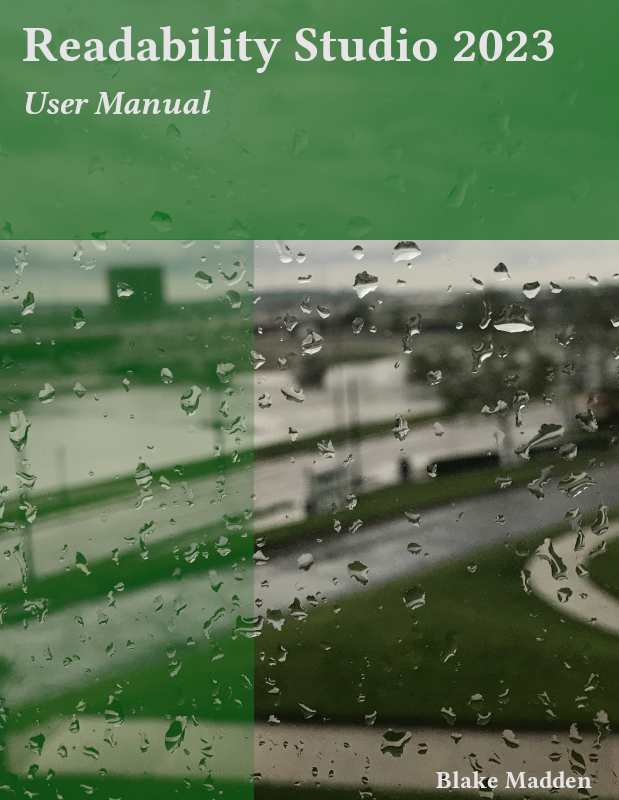
\includegraphics[width=.9\linewidth]{images/non-generated/cover.png}};
\end{tikzpicture}

% author line at the bottom
\tikz[overlay, remember picture] \node at (current page.south west)[anchor=south west]
  {
  \begin{tcolorbox}[enhanced jigsaw, sharp corners, box align=bottom, halign=right, boxsep=0.5cm,
                spread outwards, grow sidewards by=5mm,
                colback=white, colframe=white, colframe=white, opacityback=1, opacityframe=1, boxrule=0mm]
    {\fontsize{18pt}{22pt} \color{author-color} {\usefont{T1}{qcs}{b}{sc} \capitalizetitle{Blake
Madden}} }
  \end{tcolorbox}
};

\begin{tikzpicture}[overlay, remember picture]
    \node (centerimage) at (current page.south west)[anchor=south west]
    {
\includegraphics[width=3cm]{images/non-generated/cover-logo.png}};
\end{tikzpicture}

\clearpage{\thispagestyle{empty}\cleardoublepage}
\restoregeometry 

\frontmatter

\pagestyle{empty}

\begin{center}

    \topskip0pt
    \vspace*{\fill}

    \Huge \textsc{\textbf{\thetitle}} \par
    \LARGE \textit{\thesubtitle} \par

    \vspace{1cm}

    \large \theauthor

    \vspace*{\fill}

\end{center}

% reset font
    \normalfont
    \normalsize

\clearpage

\clearpage

%%%%%%%%%%%%%%%%%%%%%%%%%%%
%%%%%%%%%%%%%%%%%%%%%%%%%%%
%% Create a copyright page
%%%%%%%%%%%%%%%%%%%%%%%%%%%
%%%%%%%%%%%%%%%%%%%%%%%%%%%

\pagestyle{empty}

% Center everything
  \begin{center}

% Use Sans font
  \sffamily

% Write the Book copyright page
  \makeatletter  \small \thetitle \par \makeatother
  \makeatletter  \small \textit{\thesubtitle} \par \makeatother

% Write the CC logo, year, and author
    Copyright \ccLogo\ \makeatletter \thedate\ \theauthor \makeatother \par
    \trademark\ is a trademark of \thepublisher \par
    All rights reserved. \par

% Add a vertical space
    \vspace{0.4cm}

% Write what country it was published in
    Published in the United States

% Add a vertical space
    \vspace{0.4cm}

% Write the specific license name
    This book is distributed under a Creative Commons Attribution-Sharealike 4.0 License. \par

% Add a vertical space
    \vspace{0.4cm}

% Write the Creative Commons Icons
    \ccbysa

% Stop centering everything
  \end{center}

% Write license text
   \scriptsize
   \noindent
    That means you are free:
      \begin{itemize}
        \setlength{\itemsep}{0pt}
        \setlength{\parskip}{0pt}
        \setlength{\parsep}{0pt} 
         \item \textbf{To Share} -- copy and redistribute the material in any medium or format.
         \item \textbf{To Adapt} -- remix, transform, and build upon the material.
      \end{itemize}
    The licensor cannot revoke these freedoms as long as you follow the license terms: \par
      \begin{itemize}
        \setlength{\itemsep}{0pt}
        \setlength{\parskip}{0pt}
        \setlength{\parsep}{0pt}
          \item \textbf{Attribution} -- You must give appropriate credit, provide a link to the license, and indicate if changes were made. You may do so in any reasonable manner, but not in any way that suggests the licensor endorses you or your use. \par
          \item \textbf{Share Alike} -- If you remix, transform, or build upon the material, you must distribute your contributions under the same license as the original. \par
      \end{itemize}
    \textbf{No additional restrictions — You may not apply legal terms or technological measures that legally restrict others from doing anything the license permits.}

% reset font
    \normalfont
    \normalsize

% End the page
\clearpage

\clearpage

\pagestyle{fancy}

\renewcommand*\contentsname{Table of contents}
{
\hypersetup{linkcolor=}
\setcounter{tocdepth}{1}
\tableofcontents
}
\setstretch{1.15}

\mainmatter

\bookmarksetup{startatroot}

\chapter*{Preface}\label{sec-preface}
\addcontentsline{toc}{chapter}{Preface}

\markboth{Preface}{Preface}

This book is a guide to building, installing, and maintaining the
software product \emph{Readability Studio}.

System administrators can follow this guide for deploying installations
and updates of \emph{Readability Studio}. Additionally, instructions are
provided for system administrators and individual users for how to build
the program from source and optionally install it.

\emph{Readability Studio} is available for Microsoft\textsuperscript{®}
Windows \faWindows, macOS \faApple, and Linux \faLinux.

\part{Installing}

\chapter{\texorpdfstring{Microsoft\textsuperscript{®} Windows
\faWindows }{Microsoft® Windows }}\label{microsoft-windows}

\begin{longtable}[]{@{}
  >{\raggedright\arraybackslash}p{(\linewidth - 0\tabcolsep) * \real{1.0000}}@{}}
\toprule\noalign{}
\begin{minipage}[b]{\linewidth}\raggedright
Requirements
\end{minipage} \\
\midrule\noalign{}
\endhead
\bottomrule\noalign{}
\endlastfoot
64-bit Windows 10 (or higher) \\
x86\_64 processor \\
2 GB of RAM (4 GB recommended) \\
\end{longtable}

The \emph{Microsoft Visual C++ runtime} is also required. This is
normally managed via \emph{Windows Update}, but can also be installed
manually. To install, download and run the latest
\href{https://learn.microsoft.com/en-us/cpp/windows/latest-supported-vc-redist}{Microsoft
Visual C++ Redistributable} installer.

\section*{Installing}\label{installing-1}
\addcontentsline{toc}{section}{Installing}

\markright{Installing}

Run the installer (``rssetup2024.0.1.0.exe'') as an administrator. You
will be prompted for a user name, where to install the program, and
which components to install. After answering these prompts, continue the
installer to completion.

\section*{Updating}\label{updating}
\addcontentsline{toc}{section}{Updating}

\markright{Updating}

To upgrade an installation, run the installer
(``rssetup2024.0.1.0.exe'') as an administrator and follow the prompts.
If there is a previous installation of \emph{Readability Studio}, then
the installer will update it.

\begin{notesection}
If updating a 32-bit edition of \emph{Readability Studio} (version 2021
or earlier), you will first need to uninstall the program. The 64-bit
editions default to the 64-bit \emph{Windows} program folder, while
earlier editions where installed to the ``Program Files (x86)'' folder.
Uninstalling any 32-bit editions will ensure that you won't have
multiple installations after updating.

\end{notesection}

\newpage{}

\section*{Silent Mode}\label{silent-mode}
\addcontentsline{toc}{section}{Silent Mode}

\markright{Silent Mode}

The \emph{Readability Studio} installer uses \emph{Inno Setup}, which
provides support for silent install. (This applies to both installation
and upgrading.) To perform a silent install, pass the command line
arguments \texttt{/SILENT} or \texttt{/VERYSILENT}. For example, the
following will run a silent install that will not restart the computer
and write its progress to a log file:

\begin{Shaded}
\begin{Highlighting}[]
\ExtensionTok{rssetup.exe}\NormalTok{ /SILENT /NORESTART /LOG}
\end{Highlighting}
\end{Shaded}

\chapter{\texorpdfstring{macOS \faApple }{macOS }}\label{macos}

\begin{longtable}[]{@{}
  >{\raggedright\arraybackslash}p{(\linewidth - 0\tabcolsep) * \real{1.0000}}@{}}
\toprule\noalign{}
\begin{minipage}[b]{\linewidth}\raggedright
Requirements
\end{minipage} \\
\midrule\noalign{}
\endhead
\bottomrule\noalign{}
\endlastfoot
macOS 10.15 (or higher) \\
Apple Silicon or Intel processor \\
2 GB of RAM (4 GB recommended) \\
\end{longtable}

\section*{Installing}\label{installing-2}
\addcontentsline{toc}{section}{Installing}

\markright{Installing}

Open ``ReadabilityStudio.dmg'' and drag-and-drop the program into the
``Applications'' folder.

\section*{Updating}\label{updating-1}
\addcontentsline{toc}{section}{Updating}

\markright{Updating}

Open ``ReadabilityStudio.dmg'' and drag-and-drop the program into the
``Applications'' folder, replacing the existing copy.

\chapter{\texorpdfstring{Linux \faLinux }{Linux }}\label{linux}

\begin{longtable}[]{@{}
  >{\raggedright\arraybackslash}p{(\linewidth - 0\tabcolsep) * \real{1.0000}}@{}}
\toprule\noalign{}
\begin{minipage}[b]{\linewidth}\raggedright
Requirements
\end{minipage} \\
\midrule\noalign{}
\endhead
\bottomrule\noalign{}
\endlastfoot
x86\_64 processor \\
2 GB of RAM (4 GB recommended) \\
\end{longtable}

\section*{Installing}\label{installing-3}
\addcontentsline{toc}{section}{Installing}

\markright{Installing}

Make ``Readability\_Studio-x86\_64.AppImage'' executable. This can be
done with the following syntax:

\begin{Shaded}
\begin{Highlighting}[]
\NormalTok{chmod u}\SpecialCharTok{+}\NormalTok{x }\SpecialCharTok{\textless{}}\NormalTok{AppImage File}\SpecialCharTok{\textgreater{}}
\end{Highlighting}
\end{Shaded}

This can also be down by right-clicking the file, selecting
\menu[,]{{Properties},{Permissions}} and checking \emph{Allow executing
file as program}.

This only needs to be done once. Now
``Readability\_Studio-x86\_64.AppImage'' can be ran directly to launch
the program.

\section*{Updating}\label{updating-2}
\addcontentsline{toc}{section}{Updating}

\markright{Updating}

Replace your existing AppImage with the latest version. Make the new
AppImage executable and then it will be ready to run.

\part{Building from Source}

\chapter{\texorpdfstring{Microsoft\textsuperscript{®} Windows
\faWindows }{Microsoft® Windows }}\label{microsoft-windows-1}

\begin{longtable}[]{@{}
  >{\raggedright\arraybackslash}p{(\linewidth - 0\tabcolsep) * \real{1.0000}}@{}}
\toprule\noalign{}
\begin{minipage}[b]{\linewidth}\raggedright
Install the following tools to build \emph{Readability Studio}
\end{minipage} \\
\midrule\noalign{}
\endhead
\bottomrule\noalign{}
\endlastfoot
\emph{Visual Studio} \\
\emph{Inno Setup} \\
\emph{R} (optional) \\
\emph{Quarto} (optional) \\
\end{longtable}

Perform the following to build:

\section*{\texorpdfstring{Build
\emph{wxWidgets}}{Build wxWidgets}}\label{build-wxwidgets}
\addcontentsline{toc}{section}{Build \emph{wxWidgets}}

\markright{Build \emph{wxWidgets}}

\begin{itemize}
\tightlist
\item
  Open \emph{Visual Studio} and select \emph{Clone a Repository}

  \begin{itemize}
  \tightlist
  \item
    Enter
    \href{https://github.com/wxWidgets/wxWidgets.git}{``https://github.com/wxWidgets/wxWidgets.git''}
    and clone it
  \end{itemize}
\item
  Once the ``wxWidgets'' folder is cloned and opened in \emph{Visual
  Studio}:

  \begin{itemize}
  \tightlist
  \item
    Open \menu[,]{{Project},{CMake Settings for wxWidgets}}

    \begin{itemize}
    \tightlist
    \item
      Uncheck \textbf{wxBUILD\_SHARED}
    \item
      Set \textbf{wxBUILD\_OPTIMISE} to ``ON''
    \item
      Set the configuration type to ``Release''
    \item
      Save your changes
    \end{itemize}
  \item
    Select \menu[,]{{Build},{Install wxWidgets}} (builds and then copies
    the header, lib, and cmake files to the prefix folder)
  \end{itemize}
\end{itemize}

\newpage{}

\section*{\texorpdfstring{Build \emph{Readability
Studio}}{Build Readability Studio}}\label{build}
\addcontentsline{toc}{section}{Build \emph{Readability Studio}}

\markright{Build \emph{Readability Studio}}

\begin{itemize}
\tightlist
\item
  From \emph{Visual Studio}, select \emph{Clone a Repository} again

  \begin{itemize}
  \tightlist
  \item
    Enter
    \href{https://github.com/Blake-Madden/ReadabilityStudio.git}{``https://github.com/Blake-Madden/ReadabilityStudio.git''}
    and clone it to the same level as the ``wxWidgets'' folder
  \end{itemize}
\item
  Once the ``ReadabilityStudio'' folder is cloned and opened in
  \emph{Visual Studio}:

  \begin{itemize}
  \tightlist
  \item
    Open \menu[,]{{Project},{CMake Settings for readstudio}}

    \begin{itemize}
    \tightlist
    \item
      Set the configuration type to ``Release'' (or create a new release
      configuration)
    \item
      Save your changes
    \end{itemize}
  \end{itemize}
\item
  Select \menu[,]{{View},{CMake Targets}}
\item
  Build the ``readstudio'' target
\item
  Optionally, the ``manuals'' target can also be ran to rebuild the
  documentation
\end{itemize}

\section*{Build the installer}\label{build-the-installer}
\addcontentsline{toc}{section}{Build the installer}

\markright{Build the installer}

\begin{notesection}
If you build the ``Release'' version of \emph{Readability Studio}, then
the CMake build process will copy ``readstudio.exe'' into
\menu[,]{{installers},{windows},{release}}.

\end{notesection}

\begin{itemize}
\tightlist
\item
  Go to \menu[,]{{installers},{windows}}
\item
  Digitally sign ``release/readstudio.exe''
\item
  Open ``readstudio.iss'' in \emph{Inno Setup} and build the installer

  \begin{itemize}
  \tightlist
  \item
    The installer will be placed in ``output/rssetup2024.0.1.0.exe''
  \end{itemize}
\item
  Digitally sign the installer
\end{itemize}

\chapter{\texorpdfstring{macOS \faApple }{macOS }}\label{macos-1}

\begin{longtable}[]{@{}
  >{\raggedright\arraybackslash}p{(\linewidth - 0\tabcolsep) * \real{1.0000}}@{}}
\toprule\noalign{}
\begin{minipage}[b]{\linewidth}\raggedright
Install the following tools to build \emph{Readability Studio}
\end{minipage} \\
\midrule\noalign{}
\endhead
\bottomrule\noalign{}
\endlastfoot
\emph{XCode} \\
\emph{CMake} \\
\emph{create-dmg} \\
\emph{Homebrew} \\
\emph{R} (optional) \\
\emph{Quarto} (optional) \\
\end{longtable}

To install home-brew:

\begin{Shaded}
\begin{Highlighting}[]
\ExtensionTok{/bin/bash} \AttributeTok{{-}c} \DataTypeTok{\textbackslash{}}
    \StringTok{"}\VariableTok{$(}\ExtensionTok{curl} \AttributeTok{{-}fsSL}\NormalTok{ https://raw.githubusercontent.com/Homebrew/install/HEAD/install.sh}\VariableTok{)}\StringTok{"}
\end{Highlighting}
\end{Shaded}

To install \emph{CMake} and \emph{create-dmg}:

\begin{Shaded}
\begin{Highlighting}[]
\ExtensionTok{brew}\NormalTok{ install cmake}
\ExtensionTok{brew}\NormalTok{ install create{-}dmg}
\end{Highlighting}
\end{Shaded}

If you get errors about not finding a CXX compiler, run this:

\begin{Shaded}
\begin{Highlighting}[]
\FunctionTok{sudo}\NormalTok{ xcode{-}select }\AttributeTok{{-}{-}reset}
\end{Highlighting}
\end{Shaded}

If you are notarizing the app locally, then add a notarization keychain
to your system (\texttt{APPLE\_ID} should be set to your Apple account,
usually your email address). This only needs to be done once:

\begin{Shaded}
\begin{Highlighting}[]
\VariableTok{APPLE\_ID}\OperatorTok{=}
\ExtensionTok{xcrun}\NormalTok{ notarytool store{-}credentials }\AttributeTok{{-}{-}apple{-}id} \VariableTok{$\{APPLE\_ID\}}
\end{Highlighting}
\end{Shaded}

When prompted, set the keychain profile to a meaningful name and enter
your 10-digit organization ID as the team ID. Then enter your
app-specific password. (You can get that from Apple's developer
website.)

\newpage{}

\section*{\texorpdfstring{Build
\emph{wxWidgets}}{Build wxWidgets}}\label{build-wxwidgets-1}
\addcontentsline{toc}{section}{Build \emph{wxWidgets}}

\markright{Build \emph{wxWidgets}}

Download \emph{wxWidgets}:

\begin{Shaded}
\begin{Highlighting}[]
\FunctionTok{git}\NormalTok{ clone https://github.com/wxWidgets/wxWidgets.git }\AttributeTok{{-}{-}recurse{-}submodules}
\BuiltInTok{cd}\NormalTok{ wxWidgets}
\end{Highlighting}
\end{Shaded}

Before building \emph{wxWidgets}, a patch needs to be applied to add
text control features needed by the program. Follow the instructions in
\menu[,]{{wxpatch},{macOS},{Instructions.txt}} to apply the patch, and
then build:

\begin{Shaded}
\begin{Highlighting}[]
\FunctionTok{cmake}\NormalTok{ . }\AttributeTok{{-}DCMAKE\_INSTALL\_PREFIX}\OperatorTok{=}\NormalTok{./wxlib }\AttributeTok{{-}DwxBUILD\_SHARED}\OperatorTok{=}\NormalTok{OFF }\DataTypeTok{\textbackslash{}}
    \AttributeTok{{-}D}\StringTok{"CMAKE\_OSX\_ARCHITECTURES:STRING=arm64;x86\_64"} \DataTypeTok{\textbackslash{}}
    \AttributeTok{{-}DCMAKE\_OSX\_DEPLOYMENT\_TARGET}\OperatorTok{=}\NormalTok{10.13 }\DataTypeTok{\textbackslash{}}
    \AttributeTok{{-}DwxBUILD\_OPTIMISE}\OperatorTok{=}\NormalTok{ON }\AttributeTok{{-}DwxBUILD\_STRIPPED\_RELEASE}\OperatorTok{=}\NormalTok{ON }\AttributeTok{{-}DCMAKE\_BUILD\_TYPE}\OperatorTok{=}\NormalTok{Release}

\FunctionTok{cmake} \AttributeTok{{-}{-}build}\NormalTok{ . }\AttributeTok{{-}{-}target}\NormalTok{ install }\AttributeTok{{-}{-}config}\NormalTok{ Release}
\BuiltInTok{cd}\NormalTok{ ..}
\end{Highlighting}
\end{Shaded}

\section*{\texorpdfstring{Build \emph{Readability
Studio}}{Build Readability Studio}}\label{build-1}
\addcontentsline{toc}{section}{Build \emph{Readability Studio}}

\markright{Build \emph{Readability Studio}}

\begin{Shaded}
\begin{Highlighting}[]
\FunctionTok{git}\NormalTok{ clone https://github.com/Blake{-}Madden/ReadabilityStudio.git }\AttributeTok{{-}{-}recurse{-}submodules}
\BuiltInTok{cd}\NormalTok{ ReadabilityStudio}

\FunctionTok{cmake}\NormalTok{ . }\AttributeTok{{-}DCMAKE\_BUILD\_TYPE}\OperatorTok{=}\NormalTok{Release }\AttributeTok{{-}G}\NormalTok{ Xcode}
\CommentTok{\# XCode will not understand an "all" target,}
\CommentTok{\# so the binary and manuals must be built separately}
\FunctionTok{cmake} \AttributeTok{{-}{-}build}\NormalTok{ . }\AttributeTok{{-}{-}target}\NormalTok{ readstudio }\AttributeTok{{-}{-}config}\NormalTok{ Release}
\CommentTok{\# Uncomment to build the manuals}
\CommentTok{\#cmake {-}{-}build . {-}{-}target manuals}
\end{Highlighting}
\end{Shaded}

If code signing locally, do the following:

(\texttt{ORG\_ID} should be set to your 10-digit Apple developer
organization ID and \texttt{KEYCHAIN\_PROFILE} should be the keychain
profile connected to your Apple ID):

\begin{Shaded}
\begin{Highlighting}[]
\VariableTok{ORG\_ID}\OperatorTok{=}
\VariableTok{KEYCHAIN\_PROFILE}\OperatorTok{=}

\BuiltInTok{cd}\NormalTok{ installers/macos/release}

\ExtensionTok{codesign} \AttributeTok{{-}{-}force} \AttributeTok{{-}{-}verbose}\OperatorTok{=}\NormalTok{2 }\AttributeTok{{-}{-}options}\NormalTok{ runtime }\DataTypeTok{\textbackslash{}}
         \AttributeTok{{-}{-}timestamp} \AttributeTok{{-}{-}sign} \VariableTok{$\{ORG\_ID\}}\NormalTok{ ./}\StringTok{"Readability Studio.app"}

\ExtensionTok{codesign} \AttributeTok{{-}{-}verify} \AttributeTok{{-}{-}verbose}\OperatorTok{=}\NormalTok{2 ./}\StringTok{"Readability Studio.app"}
\end{Highlighting}
\end{Shaded}

\newpage{}

\section*{Build the DMG image}\label{build-the-dmg-image}
\addcontentsline{toc}{section}{Build the DMG image}

\markright{Build the DMG image}

\begin{notesection}
If you build the ``Release'' version of \emph{Readability Studio}, then
the CMake build process will copy ``Readability Studio.app'' into
\menu[,]{{installers},{macos},{release}}.

\end{notesection}

Go to \menu[,]{{installers},{macos},{release}} and run the following:

\begin{Shaded}
\begin{Highlighting}[]
\BuiltInTok{test} \AttributeTok{{-}f}\NormalTok{ ReadabilityStudio.dmg }\KeywordTok{\&\&} \FunctionTok{rm}\NormalTok{ ReadabilityStudio.dmg}
\ExtensionTok{create{-}dmg} \DataTypeTok{\textbackslash{}}
  \AttributeTok{{-}{-}volname} \StringTok{"Readability Studio Installer"} \DataTypeTok{\textbackslash{}}
  \AttributeTok{{-}{-}volicon} \StringTok{"../../app{-}logo.icns"} \DataTypeTok{\textbackslash{}}
  \AttributeTok{{-}{-}background} \StringTok{"../../app{-}logo.png"} \DataTypeTok{\textbackslash{}}
  \AttributeTok{{-}{-}window{-}pos}\NormalTok{ 200 120 }\DataTypeTok{\textbackslash{}}
  \AttributeTok{{-}{-}window{-}size}\NormalTok{ 800 400 }\DataTypeTok{\textbackslash{}}
  \AttributeTok{{-}{-}icon{-}size}\NormalTok{ 100 }\DataTypeTok{\textbackslash{}}
  \AttributeTok{{-}{-}icon} \StringTok{"readstudio.app"}\NormalTok{ 200 190 }\DataTypeTok{\textbackslash{}}
  \AttributeTok{{-}{-}hide{-}extension} \StringTok{"readstudio.app"} \DataTypeTok{\textbackslash{}}
  \AttributeTok{{-}{-}app{-}drop{-}link}\NormalTok{ 600 185 }\DataTypeTok{\textbackslash{}}
  \StringTok{"ReadabilityStudio.dmg"} \DataTypeTok{\textbackslash{}}
  \StringTok{"release/"}
\end{Highlighting}
\end{Shaded}

If notarizing locally, then sign, notarize, staple, and verify the DMG
image:

\begin{Shaded}
\begin{Highlighting}[]
\ExtensionTok{codesign} \AttributeTok{{-}{-}force} \AttributeTok{{-}{-}verbose}\OperatorTok{=}\NormalTok{2 }\AttributeTok{{-}{-}sign} \VariableTok{$\{ORG\_ID\}}\NormalTok{ ./ReadabilityStudio.dmg}
\ExtensionTok{codesign} \AttributeTok{{-}{-}verify} \AttributeTok{{-}{-}verbose}\OperatorTok{=}\NormalTok{2 ./ReadabilityStudio.dmg}
\ExtensionTok{hdiutil}\NormalTok{ verify ./ReadabilityStudio.dmg}
\ExtensionTok{xcrun}\NormalTok{ notarytool submit ./ReadabilityStudio.dmg }\DataTypeTok{\textbackslash{}}
  \AttributeTok{{-}{-}keychain{-}profile} \VariableTok{$\{KEYCHAIN\_PROFILE\}} \DataTypeTok{\textbackslash{}}
  \AttributeTok{{-}{-}wait}

\ExtensionTok{xcrun}\NormalTok{ stapler staple ./ReadabilityStudio.dmg}

\ExtensionTok{xcrun}\NormalTok{ spctl }\AttributeTok{{-}{-}assess} \AttributeTok{{-}{-}type}\NormalTok{ open }\AttributeTok{{-}{-}context}\NormalTok{ context:primary{-}signature }\DataTypeTok{\textbackslash{}}
            \AttributeTok{{-}{-}ignore{-}cache} \AttributeTok{{-}{-}verbose}\OperatorTok{=}\NormalTok{2 ./ReadabilityStudio.dmg}
\end{Highlighting}
\end{Shaded}

If you get a notarization error, run the following (\texttt{GUID} will
be the unique ID that the submission process just displayed):

\begin{Shaded}
\begin{Highlighting}[]
\ExtensionTok{xcrun}\NormalTok{ notarytool log }\VariableTok{$\{GUID\}} \AttributeTok{{-}{-}keychain{-}profile} \VariableTok{$\{KEYCHAIN\_PROFILE\}}
\end{Highlighting}
\end{Shaded}

\chapter{\texorpdfstring{Linux \faLinux }{Linux }}\label{linux-1}

\begin{longtable}[]{@{}
  >{\raggedright\arraybackslash}p{(\linewidth - 0\tabcolsep) * \real{1.0000}}@{}}
\toprule\noalign{}
\begin{minipage}[b]{\linewidth}\raggedright
Install the following tools to build \emph{Readability Studio}
\end{minipage} \\
\midrule\noalign{}
\endhead
\bottomrule\noalign{}
\endlastfoot
\emph{GCC} (C++ and fortran compilers) \\
\emph{CMake} \\
\emph{git} \\
\emph{AppImage} \\
\emph{linuxdeploy} \\
\emph{Homebrew} \\
\emph{R} (optional) \\
\emph{Quarto} (optional) \\
\end{longtable}

\begin{longtable}[]{@{}
  >{\raggedright\arraybackslash}p{(\linewidth - 0\tabcolsep) * \real{1.0000}}@{}}
\toprule\noalign{}
\begin{minipage}[b]{\linewidth}\raggedright
Install the following libraries (and their development files, if
mentioned)
\end{minipage} \\
\midrule\noalign{}
\endhead
\bottomrule\noalign{}
\endlastfoot
\emph{GTK 3}, \emph{gtk3-devel}/\emph{libgtk3-dev} \\
\emph{libCURL}, \emph{libcurl-devel}/\emph{libcurl-dev} \\
\emph{GStreamer}, \emph{gstreamer-devel} \\
\emph{libsecret}, \emph{libsecret-devel}/\emph{libsecret-1-dev} \\
\emph{webkit}, \emph{webkit2} \\
\emph{SDL2-devel} \\
\emph{libnotify}, \emph{libnotify-devel}/\emph{libnotify-dev} \\
\emph{TBB}, \emph{tbb-devel}/\emph{tbb-dev} \\
\emph{OpenMP} \\
\emph{libopenssl}, \emph{libopenssl-3-devel}/\emph{libssl-dev} \\
\emph{libxml2}, \emph{libxml2-devel}/\emph{libxml2-dev} \\
\end{longtable}

If building the documentation, prepare \emph{R} to install packages:

\begin{Shaded}
\begin{Highlighting}[]
\ExtensionTok{R}
\ExtensionTok{install.packages}\ErrorTok{(}\StringTok{"pacman"}\KeywordTok{)}
\end{Highlighting}
\end{Shaded}

\newpage{}

\section*{\texorpdfstring{Build
\emph{wxWidgets}}{Build wxWidgets}}\label{build-wxwidgets-2}
\addcontentsline{toc}{section}{Build \emph{wxWidgets}}

\markright{Build \emph{wxWidgets}}

\begin{Shaded}
\begin{Highlighting}[]
\FunctionTok{git}\NormalTok{ clone https://github.com/wxWidgets/wxWidgets.git }\AttributeTok{{-}{-}recurse{-}submodules}
\BuiltInTok{cd}\NormalTok{ wxWidgets}

\FunctionTok{cmake}\NormalTok{ . }\AttributeTok{{-}DCMAKE\_INSTALL\_PREFIX}\OperatorTok{=}\NormalTok{./wxlib }\AttributeTok{{-}DwxBUILD\_SHARED}\OperatorTok{=}\NormalTok{OFF }\DataTypeTok{\textbackslash{}}
        \AttributeTok{{-}DwxBUILD\_OPTIMISE}\OperatorTok{=}\NormalTok{ON }\AttributeTok{{-}DwxBUILD\_STRIPPED\_RELEASE}\OperatorTok{=}\NormalTok{ON }\AttributeTok{{-}DCMAKE\_BUILD\_TYPE}\OperatorTok{=}\NormalTok{Release}

\FunctionTok{cmake} \AttributeTok{{-}{-}build}\NormalTok{ . }\AttributeTok{{-}{-}target}\NormalTok{ install }\AttributeTok{{-}j} \VariableTok{$(}\FunctionTok{nproc}\VariableTok{)} \AttributeTok{{-}{-}config}\NormalTok{ Release}
\BuiltInTok{cd}\NormalTok{ ..}
\end{Highlighting}
\end{Shaded}

\section*{\texorpdfstring{Build \emph{Readability
Studio}}{Build Readability Studio}}\label{build-2}
\addcontentsline{toc}{section}{Build \emph{Readability Studio}}

\markright{Build \emph{Readability Studio}}

\begin{Shaded}
\begin{Highlighting}[]
\FunctionTok{git}\NormalTok{ clone https://github.com/Blake{-}Madden/ReadabilityStudio.git }\AttributeTok{{-}{-}recurse{-}submodules}
\BuiltInTok{cd}\NormalTok{ ReadabilityStudio}

\FunctionTok{cmake}\NormalTok{ . }\AttributeTok{{-}DCMAKE\_BUILD\_TYPE}\OperatorTok{=}\NormalTok{Release}
\CommentTok{\# Instead of "readstudio", target can also be "manuals" to build}
\CommentTok{\# the help or "all" to build the program and help}
\FunctionTok{cmake} \AttributeTok{{-}{-}build}\NormalTok{ . }\AttributeTok{{-}{-}target}\NormalTok{ readstudio }\AttributeTok{{-}j} \VariableTok{$(}\FunctionTok{nproc}\VariableTok{)} \AttributeTok{{-}{-}config}\NormalTok{ Release}
\end{Highlighting}
\end{Shaded}

\section*{Build the AppImage}\label{build-the-appimage}
\addcontentsline{toc}{section}{Build the AppImage}

\markright{Build the AppImage}

\begin{Shaded}
\begin{Highlighting}[]
\ExtensionTok{linuxdeploy{-}x86\_64.AppImage} \AttributeTok{{-}{-}appdir}\NormalTok{ installers/unix/AppDir }\DataTypeTok{\textbackslash{}}
  \AttributeTok{{-}{-}executable}\NormalTok{ installers/unix/AppDir/usr/bin/readstudio }\DataTypeTok{\textbackslash{}}
  \AttributeTok{{-}d}\NormalTok{ installers/unix/AppDir/readstudio.desktop }\DataTypeTok{\textbackslash{}}
  \AttributeTok{{-}i}\NormalTok{ installers/unix/AppDir/app{-}logo.svg }\DataTypeTok{\textbackslash{}}
  \AttributeTok{{-}{-}output}\NormalTok{ appimage}
\FunctionTok{mv}\NormalTok{ Readability\_Studio}\PreprocessorTok{*}\NormalTok{.AppImage ./installers/unix}
\end{Highlighting}
\end{Shaded}

Once built, the AppImage will be available in
\menu[,]{{installers},{unix}}. Apply a GPG signature to it before
distributing.

\backmatter

\begingroup
% 1.5 spacing just for the citation page
\setstretch{1.5}
\printbibliography[title=References,heading=bibintoc]
\endgroup


%% Index
\printindex

\clearpage{\thispagestyle{empty}\cleardoublepage}

%% Author bio at the end

\end{document}
